\documentclass[aspectratio=169]{beamer}
\usetheme{Madrid}
\usecolortheme{whale}
\usefonttheme{professionalfonts}

\usepackage{amsmath, amssymb}
\usepackage{bm}
\usepackage{booktabs}
\usepackage{graphicx}
\usepackage{xcolor}
\usepackage{tikz}
\usetikzlibrary{arrows.meta, positioning, calc}

\setbeamertemplate{navigation symbols}{}
\setbeamertemplate{footline}[frame number]
\setbeamercolor{block title}{bg=blue!70!black,fg=white}
\setbeamercolor{block body}{bg=blue!8}
\setbeamercolor{alertblock title}{bg=red!70!black,fg=white}
\setbeamercolor{alertblock body}{bg=red!8}
\setbeamercolor{exampleblock title}{bg=green!60!black,fg=white}
\setbeamercolor{exampleblock body}{bg=green!8}

\title[Networks, FX Policy, SOE]{Networks, Exchange Rates, and Monetary Policy\\
in a Small Open Economy}
\subtitle{Extending Rubbo (2024) to FX Regime Analysis}
\author{[Your Name]}
\institute{[Your Institution]}
\date{July 22, 2026}

\begin{document}

%---------------------------------------------------------------
\begin{frame}
\titlepage
\end{frame}

%---------------------------------------------------------------
\begin{frame}{Outline}
\tableofcontents
\end{frame}

%==============================================================
\section{Motivation}
%==============================================================

\begin{frame}{Motivation: Two Puzzles}
\begin{columns}
\begin{column}{0.48\textwidth}
\begin{block}{Puzzle 1: Which Inflation to Target?}
\begin{itemize}
    \item Multi-sector economies: CPI includes many sectors with different stickiness
    \item Rubbo (2024): optimal target is \textit{not} CPI --- it is a network-adjusted index
    \item \textbf{Q: How does this change in an open economy?}
\end{itemize}
\end{block}
\end{column}
\begin{column}{0.48\textwidth}
\begin{block}{Puzzle 2: Float vs.\ Peg?}
\begin{itemize}
    \item Exchange rate movements propagate through supply chains
    \item Sectors with upstream import linkages amplify pass-through
    \item \textbf{Q: What FX regime minimizes welfare loss in a networked economy?}
\end{itemize}
\end{block}
\end{column}
\end{columns}

\vspace{0.4cm}
\begin{alertblock}{This Paper}
We extend Rubbo (2024) to a small open economy and show:
\begin{enumerate}
    \item The ``divine coincidence'' breaks down under a float (two cost-push channels)
    \item Network structure determines optimal FX policy
    \item Countries with heterogeneous import intensity benefit most from FX intervention
\end{enumerate}
\end{alertblock}
\end{frame}

%---------------------------------------------------------------
\begin{frame}{Roadmap}
\begin{center}
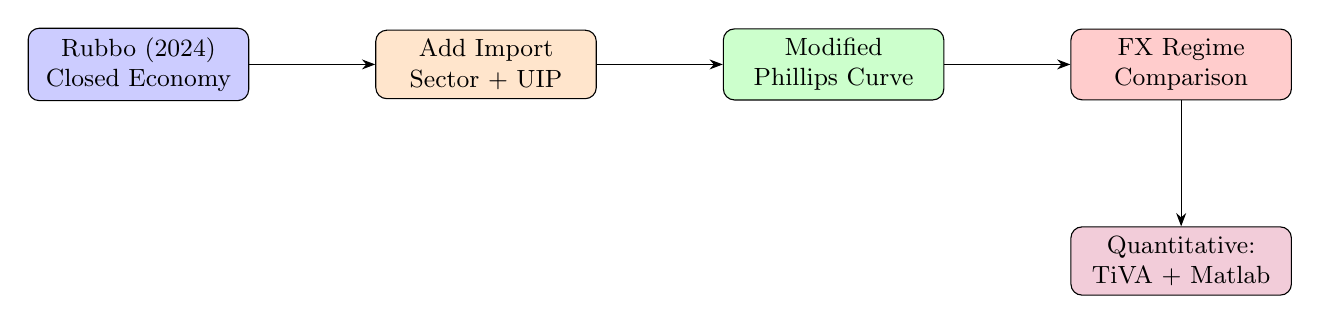
\begin{tikzpicture}[node distance=1.6cm, every node/.style={rounded corners, align=center, font=\small}]
    \node[draw,fill=blue!20,minimum width=2.8cm,minimum height=0.8cm] (A) {Rubbo (2024)\\Closed Economy};
    \node[draw,fill=orange!20,minimum width=2.8cm,minimum height=0.8cm, right=of A] (B) {Add Import\\Sector + UIP};
    \node[draw,fill=green!20,minimum width=2.8cm,minimum height=0.8cm, right=of B] (C) {Modified\\Phillips Curve};
    \node[draw,fill=red!20,minimum width=2.8cm,minimum height=0.8cm, right=of C] (D) {FX Regime\\Comparison};
    \node[draw,fill=purple!20,minimum width=2.8cm,minimum height=0.8cm, below=of D] (E) {Quantitative:\\TiVA + Matlab};
    \draw[-{Stealth}] (A) -- (B);
    \draw[-{Stealth}] (B) -- (C);
    \draw[-{Stealth}] (C) -- (D);
    \draw[-{Stealth}] (D) -- (E);
\end{tikzpicture}
\end{center}

\vspace{0.3cm}
\textbf{Key building blocks from Rubbo (2024):}
\begin{itemize}
    \item Domar weights, Leontief inverse, rigidity-adjusted network
    \item Divine coincidence index, sector-level Phillips curves
    \item Welfare: output gap + within-sector + cross-sector misallocation
\end{itemize}
\end{frame}

%==============================================================
\section{Literature Review}
%==============================================================

\begin{frame}{Literature: Three Intersecting Areas}
\begin{columns}
\begin{column}{0.32\textwidth}
\begin{block}{\small Area 1: Networks \& MP}
\small
\begin{itemize}
    \item Rubbo (2024, Ecta): sector Phillips curves, DC index
    \item La'O \& Tahbaz-Salehi (2022, Ecta): optimal MP in networks
    \item Pasten-Schoenle-Weber (2020, JME): heterogeneous Calvo + networks
    \item Baqaee \& Farhi (2020, QJE): misallocation in networks
    \item Acemoglu et al.\ (2012, Ecta): micro shocks $\to$ macro
\end{itemize}
\end{block}
\end{column}
\begin{column}{0.32\textwidth}
\begin{block}{\small Area 2: Intl.\ Networks + ER}
\small
\begin{itemize}
    \item Auer-Levchenko-Sauré (2019, REStat): IO spillovers of inflation
    \item Amiti-Itskhoki-Konings (2019, ReStud): markups + pass-through
    \item Gopinath \& Itskhoki (2022): dominant currency paradigm
    \item Bems \& Johnson (2017, AEJMacro): value-added REERs
    \item GVC literature: networks dampen pass-through
\end{itemize}
\end{block}
\end{column}
\begin{column}{0.32\textwidth}
\begin{block}{\small Area 3: FX Policy}
\small
\begin{itemize}
    \item Galí \& Monacelli (2005, ReStud): baseline SOE NK model
    \item Corsetti-Dedola-Leduc (2010): optimal MP in open economies
    \item Fanelli \& Straub (2021, ReStud): FX intervention theory
    \item Schmitt-Grohé \& Uribe (2016, JPE): peg + wage rigidity
    \item Qiu et al.\ (2026, JME): MP + production networks in open econ.
\end{itemize}
\end{block}
\end{column}
\end{columns}
\end{frame}

%---------------------------------------------------------------
\begin{frame}{Our Contribution vs.\ Existing Literature}
\begin{center}
\small
\begin{tabular}{lccc}
\toprule
& Networks & Open Econ. & FX Policy \\
\midrule
Rubbo (2024) & \checkmark & $\times$ & $\times$ \\
La'O \& Tahbaz-Salehi (2022) & \checkmark & $\times$ & $\times$ \\
Galí \& Monacelli (2005) & $\times$ & \checkmark & \checkmark \\
Fanelli \& Straub (2021) & $\times$ & \checkmark & \checkmark \\
Qiu et al.\ (2026) & \checkmark & \checkmark & $\times$ \\
Auer et al.\ (2019) & \checkmark & \checkmark & $\times$ \\
\midrule
\textbf{This paper} & \checkmark & \checkmark & \checkmark \\
\bottomrule
\end{tabular}
\end{center}

\vspace{0.3cm}
\begin{exampleblock}{Key gap we fill}
No paper combines: (i) full network structure with sector-level Phillips curves, (ii) a small open economy, \textit{and} (iii) an analysis of FX policy regimes in terms of the divine coincidence/welfare.
\end{exampleblock}
\end{frame}

%==============================================================
\section{Closed-Economy Model: Rubbo (2024)}
%==============================================================

\begin{frame}{Model: Production Network}
\begin{columns}
\begin{column}{0.55\textwidth}
\textbf{$N$ sectors}, each a continuum of Calvo firms:
\begin{align*}
    Y_{if} &= A_i F_i(L_{if}, \{X_{ijf}\}) \quad \text{(CRS)}\\
    P_i &= \left(\int P_{if}^{1-\varepsilon_i} df\right)^{1/(1-\varepsilon_i)}
\end{align*}

\textbf{Network notation:}
\begin{itemize}
    \item $\omega_{ij}$ = cost share of input $j$ in sector $i$ (IO matrix $\Omega$)
    \item $\alpha_i$ = labor cost share in sector $i$
    \item $\beta_i$ = household spending share on sector $i$
    \item $\hat{\delta}_i$ = effective Calvo frequency (price flexibility)
\end{itemize}
\end{column}
\begin{column}{0.42\textwidth}
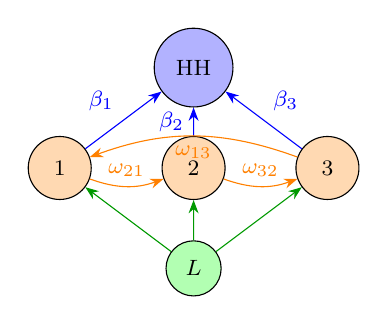
\begin{tikzpicture}[scale=0.85, every node/.style={font=\footnotesize}]
    \node[draw,circle,fill=blue!30,minimum size=1cm] (H) at (3,3.5) {HH};
    \node[draw,circle,fill=orange!30,minimum size=0.8cm] (1) at (1,2) {$1$};
    \node[draw,circle,fill=orange!30,minimum size=0.8cm] (2) at (3,2) {$2$};
    \node[draw,circle,fill=orange!30,minimum size=0.8cm] (3) at (5,2) {$3$};
    \node[draw,circle,fill=green!30,minimum size=0.7cm] (L) at (3,0.5) {$L$};
    \draw[-{Stealth},blue] (1) -- node[above left]{$\beta_1$} (H);
    \draw[-{Stealth},blue] (2) -- node[left]{$\beta_2$} (H);
    \draw[-{Stealth},blue] (3) -- node[above right]{$\beta_3$} (H);
    \draw[-{Stealth},orange] (1) to[bend right=20] node[above]{$\omega_{21}$} (2);
    \draw[-{Stealth},orange] (2) to[bend right=20] node[above]{$\omega_{32}$} (3);
    \draw[-{Stealth},orange] (3) to[bend right=20] node[below]{$\omega_{13}$} (1);
    \draw[-{Stealth},green!60!black] (L) -- (1);
    \draw[-{Stealth},green!60!black] (L) -- (2);
    \draw[-{Stealth},green!60!black] (L) -- (3);
\end{tikzpicture}
\end{column}
\end{columns}
\end{frame}

%---------------------------------------------------------------
\begin{frame}{Key Objects: Leontief Inverse and Domar Weights}

\begin{block}{Log-linearized Marginal Cost}
\begin{equation*}
    \bm{mc}_t = \underbrace{\bm{\alpha} w_t}_{\text{labor cost}} + \underbrace{\Omega\bm{p}_t}_{\text{input cost}} - \underbrace{\log\mathbf{A}_t}_{\text{TFP}}
\end{equation*}
\end{block}

\begin{columns}
\begin{column}{0.48\textwidth}
\begin{block}{Leontief Inverse}
\begin{equation*}
    (I-\Omega)^{-1} = I + \Omega + \Omega^2 + \cdots
\end{equation*}
$(I-\Omega)^{-1}_{ij}$ = total exposure of $i$'s cost to $j$'s price, through \textit{all} supply chain paths.
\end{block}
\end{column}
\begin{column}{0.48\textwidth}
\begin{block}{Domar Weights}
\begin{equation*}
    \bm{\lambda}^T = \bm{\beta}^T(I-\Omega)^{-1}
\end{equation*}
$\lambda_i$ = sector $i$'s total sales share (direct to consumers + indirect through other producers). Always $\sum_i \lambda_i > 1$.
\end{block}
\end{column}
\end{columns}

\vspace{0.3cm}
\begin{exampleblock}{Rigidity-Adjusted Leontief $(I-\Omega\Delta)^{-1}$}
Weights each step of the supply chain by sector's price flexibility $\hat{\delta}_i$. Sticky-price sectors absorb cost shocks into markups rather than prices --- they are ``discounted'' in propagation.
\end{exampleblock}
\end{frame}

%---------------------------------------------------------------
\begin{frame}{Three Lemmas (Rubbo 2024)}

\begin{block}{Lemma 1: Natural Output = Domar-Weighted TFP}
\begin{equation*}
    y_{t,\mathrm{nat}} = \frac{1+\varphi}{\gamma+\varphi}\,\bm{\lambda}^T \log\mathbf{A}_t
\end{equation*}
Natural output is a weighted sum of TFPs; weights = Domar weights (network centrality).
\end{block}

\begin{block}{Lemma 2: Output Gap = Employment Gap}
\begin{equation*}
    \tilde{y}_t = y_t - y_{t,\mathrm{nat}} = l_t - l_{t,\mathrm{nat}} = \tilde{l}_t
\end{equation*}
Because labor is allocated efficiently \textit{given} aggregate $L_t$ (envelope theorem).
\end{block}

\begin{block}{Lemma 3: Output Gap = $-$Sales-Weighted Markup}
\begin{equation*}
    (\gamma+\varphi)\tilde{y}_t = -\bm{\lambda}^T\bm{\mu}_t = -\sum_i \lambda_i \mu_{it}
\end{equation*}
Positive markups distort labor supply. Effect is amplified for sectors with high Domar weight.
\end{block}
\end{frame}

%---------------------------------------------------------------
\begin{frame}{Proposition 2: Sector-Level Phillips Curves}

\begin{equation*}
    \bm{\pi}_t = \underbrace{\rho(I-\mathcal{V})\mathbb{E}\bm{\pi}_{t+1}}_{\text{forward-looking}} + \underbrace{\mathcal{B}(\gamma+\varphi)\tilde{y}_t}_{\text{output gap}} - \underbrace{\mathcal{V}\bm{\chi}_t}_{\text{cost-push}}
\end{equation*}

\begin{columns}
\begin{column}{0.48\textwidth}
\begin{itemize}
    \item $\mathcal{B} = \dfrac{\Delta(I-\Omega\Delta)^{-1}\bm{\alpha}}{1 - \bm{\beta}^T\Delta(I-\Omega\Delta)^{-1}\bm{\alpha}}$\\[4pt]
    Phillips curve slope (network-adjusted labor share)
    \vspace{4pt}
    \item $\mathcal{V}$: cost-push matrix (rows sum to 0)\\
    Only \textit{relative} productivity matters
\end{itemize}
\end{column}
\begin{column}{0.48\textwidth}
\begin{itemize}
    \item $(I-\Omega\Delta)^{-1}$: rigidity-adjusted Leontief\\[4pt]
    Sticky sectors dampen cost propagation
    \vspace{4pt}
    \item $\bm{\chi}_t = (I-\Omega)^{-1}\log\mathbf{A}_t - \bm{p}_{t-1}$\\[4pt]
    Cost-push = efficiency-adjusted price wedge
\end{itemize}
\end{column}
\end{columns}

\vspace{0.3cm}
\begin{alertblock}{Key: Sherman-Morrison identity}
The complex matrix inversion in the proof uses: $(I - \mathbf{u}\mathbf{v}^T)^{-1} = I + \frac{\mathbf{u}\mathbf{v}^T}{1-\mathbf{v}^T\mathbf{u}}$, allowing closed-form solution for $\mathcal{B}$ and $\mathcal{V}$.
\end{alertblock}
\end{frame}

%---------------------------------------------------------------
\begin{frame}{Proposition 1: Divine Coincidence Index}

\begin{block}{Definition}
\begin{equation*}
    \pi_t^{DC} \equiv \sum_i \underbrace{\frac{\lambda_i(1-\hat{\delta}_i)/\hat{\delta}_i}{\sum_j \lambda_j(1-\hat{\delta}_j)/\hat{\delta}_j}}_{=\, w_i^{DC}} \pi_{it}
\end{equation*}
Weight $\propto$ Domar weight $\times$ price stickiness. Stickier sectors get \textit{more} weight.
\end{block}

\begin{exampleblock}{The DC Phillips Curve: No Cost-Push!}
\begin{equation*}
    \pi_t^{DC} = \rho\,\mathbb{E}\pi_{t+1}^{DC} + \underbrace{\frac{\gamma+\varphi}{\sum_j \lambda_j(1-\hat{\delta}_j)/\hat{\delta}_j}}_{\kappa_{DC}}\tilde{y}_t
\end{equation*}
\end{exampleblock}

\begin{columns}
\begin{column}{0.5\textwidth}
\textbf{Uniqueness:} $\pi^{DC}$ is the \textit{unique} inflation index with no cost-push term (one-dimensional left null space of $\mathcal{V}$).
\end{column}
\begin{column}{0.48\textwidth}
\textbf{Policy implication:} Replace CPI with $\pi^{DC}$ in the Taylor rule $\Rightarrow$ zero output gap at all times.
\end{column}
\end{columns}
\end{frame}

%---------------------------------------------------------------
\begin{frame}{Welfare (Proposition 3)}

\begin{equation*}
    \mathbb{W} = \frac{1}{2}\sum_t \rho^t \left[\underbrace{(\gamma+\varphi)\tilde{y}_t^2}_{\text{(1) output gap}} + \underbrace{\sum_i \lambda_i \frac{1-\hat{\delta}_i}{\hat{\delta}_i}\varepsilon_i\pi_{it}^2}_{\text{(2) within-sector}} + \underbrace{\Phi_C + \sum_s\lambda_s\Phi_s}_{\text{(3) cross-sector}}\right]
\end{equation*}

\vspace{0.2cm}
\begin{enumerate}
    \item \textbf{Output gap:} Same as one-sector NK model. Labor-leisure distortion.
    \vspace{0.1cm}
    \item \textbf{Within-sector price dispersion:} Under Calvo, variance of prices within sector $i$ $\approx (1-\hat{\delta}_i)\pi_{it}^2/\hat{\delta}_i$. Consumers buy from cheap (not productive) varieties.
    \vspace{0.1cm}
    \item \textbf{Cross-sector misallocation:} Relative price wedges cause inefficient substitution across sectors. Captured by Baqaee-Farhi substitution operators $\Phi$.
\end{enumerate}

\vspace{0.2cm}
\begin{alertblock}{Key implication}
Even if output gap = 0, the CB should care about \textit{which} sectors' prices inflate, because sectors differ in stickiness and network position.
\end{alertblock}
\end{frame}

%==============================================================
\section{Small Open Economy Extension}
%==============================================================

\begin{frame}{Open Economy: Modified Environment}
\begin{columns}
\begin{column}{0.55\textwidth}
\textbf{Add foreign sector $F$:}
\begin{itemize}
    \item Consumption basket: $C_t = \mathcal{C}(C_t^H, C_t^F)$
    \item CPI: $p_t^C = \mathcal{P}(p_t^H, e_t + p_t^*)$
    \item $e_t$ = log nominal exchange rate (domestic/foreign)
    \item $p_t^*$ = foreign price level (exogenous)
\end{itemize}

\vspace{0.3cm}
\textbf{Domestic firms use imports:}
\begin{equation*}
    \bm{mc}_t = \bm{\alpha}w_t + \Omega\bm{p}_t + \underbrace{\bm{\omega}_F(p_t^* + e_t)}_{\text{new term}} - \log\mathbf{A}_t
\end{equation*}
$\omega_{Fi}$ = import input share of sector $i$ (from TiVA data).
\end{column}
\begin{column}{0.42\textwidth}
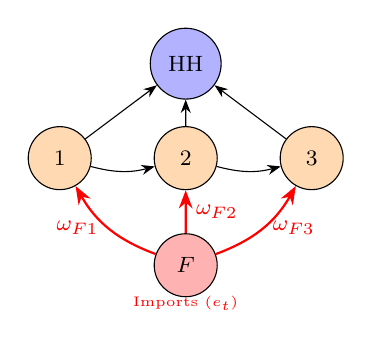
\begin{tikzpicture}[scale=0.8, every node/.style={font=\footnotesize}]
    \node[draw,circle,fill=blue!30,minimum size=0.9cm] (H) at (3,4) {HH};
    \node[draw,circle,fill=orange!30,minimum size=0.8cm] (1) at (1,2.5) {$1$};
    \node[draw,circle,fill=orange!30,minimum size=0.8cm] (2) at (3,2.5) {$2$};
    \node[draw,circle,fill=orange!30,minimum size=0.8cm] (3) at (5,2.5) {$3$};
    \node[draw,circle,fill=red!30,minimum size=0.8cm] (F) at (3,0.8) {$F$};
    \node[font=\tiny,red] at (3,0.2) {Imports ($e_t$)};
    \draw[-{Stealth}] (1) -- (H);
    \draw[-{Stealth}] (2) -- (H);
    \draw[-{Stealth}] (3) -- (H);
    \draw[-{Stealth}] (1) to[bend right=15] (2);
    \draw[-{Stealth}] (2) to[bend right=15] (3);
    \draw[-{Stealth},red,thick] (F) -- node[right]{$\omega_{F2}$} (2);
    \draw[-{Stealth},red,thick] (F) to[bend left=20] node[left]{$\omega_{F1}$} (1);
    \draw[-{Stealth},red,thick] (F) to[bend right=20] node[right]{$\omega_{F3}$} (3);
\end{tikzpicture}
\end{column}
\end{columns}

\vspace{0.2cm}
\textbf{Uncovered Interest Parity (UIP):} $i_t - i_t^* = \mathbb{E}_t\Delta e_{t+1}$
\end{frame}

%---------------------------------------------------------------
\begin{frame}{Modified Phillips Curve}

\begin{exampleblock}{Phillips Curve with Exchange Rate Pass-Through}
\begin{equation*}
    \bm{\pi}_t = \rho(I-\mathcal{V})\mathbb{E}\bm{\pi}_{t+1} + \mathcal{B}(\gamma+\varphi)\tilde{y}_t - \mathcal{V}\bm{\chi}_t + \underbrace{\Gamma\Delta e_t}_{\textbf{new}}
\end{equation*}
\end{exampleblock}

\begin{block}{Exchange Rate Pass-Through Vector}
\begin{equation*}
    \Gamma \equiv \frac{\Delta(I-\Omega\Delta)^{-1}\bm{\omega}_F}{1 - \bm{\beta}^T\Delta(I-\Omega\Delta)^{-1}\bm{\alpha}}
\end{equation*}
\end{block}

\textbf{Interpretation of $\Gamma_i$:}
\begin{itemize}
    \item Direct effect: sector $i$'s own import intensity $\omega_{Fi}$
    \item \textbf{Network amplification:} $(I-\Omega\Delta)^{-1}$ adds indirect effects through upstream suppliers' import intensity
    \item Sectors with stickier prices ($\hat{\delta}_i$ small) absorb more into markups: smaller $\Gamma_i$
    \item Sectors with many import-intensive upstream suppliers: larger $\Gamma_i$
\end{itemize}
\end{frame}

%---------------------------------------------------------------
\begin{frame}{Network Amplification of FX Pass-Through}

\textbf{Expand the rigidity-adjusted Leontief:}
\begin{equation*}
    (I-\Omega\Delta)^{-1}\bm{\omega}_F = \bm{\omega}_F + \Omega\Delta\bm{\omega}_F + (\Omega\Delta)^2\bm{\omega}_F + \cdots
\end{equation*}

\begin{center}
\small
\begin{tabular}{ll}
\toprule
\textbf{Term} & \textbf{Interpretation} \\
\midrule
$\bm{\omega}_F$ & Direct import intensity of each sector \\
$\Omega\Delta\bm{\omega}_F$ & Import intensity of direct suppliers, weighted by their price flexibility \\
$(\Omega\Delta)^2\bm{\omega}_F$ & Import intensity of suppliers' suppliers \\
$\vdots$ & \ldots \\
\bottomrule
\end{tabular}
\end{center}

\vspace{0.3cm}
\begin{alertblock}{Key Testable Prediction}
Sectors with high \textbf{upstream} import intensity (even if their own $\omega_{Fi}$ is low) experience large inflation responses to exchange rate movements. This is the network amplification effect, measurable from TiVA data.
\end{alertblock}
\end{frame}

%---------------------------------------------------------------
\begin{frame}{Result 1: Breakdown of Divine Coincidence}

\textbf{Under a float:} we need a weighting $\bm{\phi}$ such that $\bm{\phi}^T\bm{\pi}_t$ has no cost-push.

Two conditions must hold simultaneously:
\begin{equation*}
    \underbrace{\bm{\phi}^T\mathcal{V} = \mathbf{0}^T}_{\text{no productivity cost-push}} \quad \text{AND} \quad \underbrace{\bm{\phi}^T\Gamma = 0}_{\text{no ER cost-push}}
\end{equation*}

\begin{columns}
\begin{column}{0.48\textwidth}
\begin{alertblock}{Closed economy (Rubbo)}
One condition $\Rightarrow$ unique solution: the DC index $\bm{\phi}^{DC}$. \textbf{Divine coincidence holds.}
\end{alertblock}
\end{column}
\begin{column}{0.48\textwidth}
\begin{alertblock}{Open economy (this paper)}
Two conditions, one free parameter. \textbf{Generically no solution} --- unless $\Gamma \propto \mathcal{B}$ (ER affects sectors exactly like wages do). \textbf{Divine coincidence breaks down.}
\end{alertblock}
\end{column}
\end{columns}

\vspace{0.3cm}
\begin{exampleblock}{Proposition (informal)}
Under a flexible exchange rate, there is an irreducible tradeoff between output gap stability and inflation stability. The severity of the tradeoff is governed by $|\Gamma - \mathcal{B} \cdot c|$ for any scalar $c$.
\end{exampleblock}
\end{frame}

%---------------------------------------------------------------
\begin{frame}{FX Regime Comparison}

\begin{center}
\begin{tabular}{lccc}
\toprule
\textbf{Property} & \textbf{Float} & \textbf{Peg} & \textbf{Managed Float} \\
\midrule
ER cost-push $\Gamma\Delta e_t$ & Yes & Zero & Reduced \\
MP independence & Full & None & Partial \\
DC index survives? & No & Yes (trivially) & Depends on $\nu_t$ \\
Optimal inflation target & No single index & DC (can't use it) & Modified DC \\
\midrule
\textbf{Welfare} & & & \\
\quad Output gap loss & Low (can target) & High (trilemma) & Intermediate \\
\quad ER misallocation & High & Zero & Low \\
\quad Total & ? & ? & Best? \\
\bottomrule
\end{tabular}
\end{center}

\vspace{0.2cm}
\begin{block}{Trilemma (Mundell)}
Under a peg: $\Delta e_t = 0$ eliminates ER cost-push. But $i_t = i_t^*$ by UIP: CB loses monetary policy independence. Cannot close output gap. Cross-sector misallocation from foreign shocks becomes the main welfare cost.
\end{block}
\end{frame}

%---------------------------------------------------------------
\begin{frame}{Result 2: Optimal FX Intervention}

\textbf{Under a managed float:} CB has two instruments --- interest rate $i_t$ + FX intervention $\nu_t$.

\begin{block}{Optimal Policy}
\begin{enumerate}
    \item Use $i_t$ to close the output gap ($\tilde{y}_t = 0$)
    \item Use $\nu_t$ to offset the ER cost-push component that is orthogonal to $\mathcal{B}$:
    \begin{equation*}
        \nu_t^* = -\frac{\bm{\phi}^{DC,T}\Gamma}{\bm{\phi}^{DC,T}\Gamma_\nu}\,\Delta e_t^{\text{unmanaged}}
    \end{equation*}
    where $\Gamma_\nu$ is the pass-through of FX intervention to exchange rate
\end{enumerate}
\end{block}

\begin{exampleblock}{Intuition}
The CB should ``lean against'' exchange rate movements in proportion to their network-amplified pass-through. The optimal intervention depends on $\Gamma$ --- which depends on the country's IO structure and import intensity distribution $\bm{\omega}_F$.
\end{exampleblock}

\begin{alertblock}{Heterogeneity across countries}
Countries with high and \textit{heterogeneous} $\omega_{Fi}$ across sectors face worse float-peg tradeoffs (large $\Gamma$, badly-positioned). They benefit most from FX intervention.
\end{alertblock}
\end{frame}

%---------------------------------------------------------------
\begin{frame}{Modified Welfare in the Open Economy}

\begin{equation*}
    \mathbb{W}^{\text{open}} = \underbrace{\mathbb{W}^{\text{closed}}}_{\text{Rubbo (2024)}} + \underbrace{\frac{1}{2}\sum_t \rho^t \left[\Phi_C(\tilde{\bm{\chi}}_t, e_t\bm{\omega}_F) + \sum_s\lambda_s\Phi_s(\tilde{\bm{\chi}}_t, e_t\bm{\omega}_F)\right]}_{\text{ER-driven cross-sector misallocation (new)}}
\end{equation*}

\vspace{0.2cm}
\textbf{New term:} Exchange rate movements cause relative price distortions across sectors with different import intensities $\omega_{Fi}$. When the ER depreciates, import-intensive sectors face higher costs than others; relative prices diverge from efficient levels.

\vspace{0.2cm}
\begin{block}{Counterfactual: What Would CPI Targeting Do?}
\begin{itemize}
    \item CPI targeting ignores within-sector dispersion and cross-sector misallocation
    \item Under a float + CPI targeting: both output gap and ER misallocation accumulate
    \item Rubbo shows: welfare loss of 2.9--3.8\% of GDP vs.\ optimal even in \textit{closed} economy
    \item Our conjecture: losses are larger under a float, especially for countries with high $\|\Gamma\|$
\end{itemize}
\end{block}
\end{frame}

%==============================================================
\section{Data and Quantitative Strategy}
%==============================================================

\begin{frame}{Data: OECD TiVA and Country Selection}

\begin{columns}
\begin{column}{0.52\textwidth}
\textbf{OECD Trade in Value Added (TiVA):}
\begin{itemize}
    \item Inter-country IO tables, 66 countries, 45 sectors
    \item Covers: $\Omega$ (domestic IO), $\bm{\omega}_F$ (import shares by sector), $\bm{\beta}$ (consumption shares), $\bm{\lambda}$ (Domar weights)
    \item Years: 2005, 2010, 2015, 2018 (latest)
\end{itemize}

\vspace{0.3cm}
\textbf{Country selection criteria:}
\begin{itemize}
    \item Small open economy (GDP $<$ 1\% of world)
    \item Heterogeneous FX regimes (float, peg, managed)
    \item Rich IO data
    \item Candidate: South Korea, Chile, Czech Republic, New Zealand, Singapore
\end{itemize}
\end{column}
\begin{column}{0.45\textwidth}
\begin{block}{Key Parameters to Calibrate}
\begin{itemize}
    \item $\Omega$: from TiVA domestic IO table
    \item $\bm{\omega}_F$: import use by sector (TiVA)
    \item $\bm{\beta}$: final consumption shares (TiVA)
    \item $\hat{\bm{\delta}}$: sectoral Calvo frequencies from Nakamura-Steinsson (2008) mapped to TiVA sectors
    \item $\varepsilon_i$: substitution elasticities from literature
    \item $\gamma=1, \varphi=2$: standard NK calibration
    \item $\rho = 0.9975$: quarterly discount factor
\end{itemize}
\end{block}
\end{column}
\end{columns}
\end{frame}

%---------------------------------------------------------------
\begin{frame}{Quantitative Objects of Interest}

\textbf{1. Pass-through vector $\Gamma$ (theory $\to$ data):}
\begin{equation*}
    \Gamma = \frac{\Delta(I-\Omega\Delta)^{-1}\bm{\omega}_F}{1 - \bm{\beta}^T\Delta(I-\Omega\Delta)^{-1}\bm{\alpha}}
\end{equation*}
Compare direct import intensity $\bm{\omega}_F$ vs.\ network-amplified $\Gamma$: how much does the network matter?

\vspace{0.2cm}
\textbf{2. DC index weights (country comparison):}
\begin{equation*}
    w_i^{DC} = \frac{\lambda_i(1-\hat{\delta}_i)/\hat{\delta}_i}{\sum_j\lambda_j(1-\hat{\delta}_j)/\hat{\delta}_j}
\end{equation*}
How much do DC weights differ from CPI weights? How much do they differ across countries?

\vspace{0.2cm}
\textbf{3. Welfare comparison across FX regimes (simulation):}
\begin{itemize}
    \item Simulate model under Float / Peg / Managed Float
    \item Compute $\mathbb{W}^{\text{open}}$ for each regime, for each country
    \item Identify: which countries should float? Which should peg?
\end{itemize}
\end{frame}

%---------------------------------------------------------------
\begin{frame}{Matlab Simulation Plan}

\textbf{Extends Rubbo's existing code (\texttt{replication files/calibration/}):}

\begin{center}
\small
\begin{tabular}{lll}
\toprule
\textbf{Task} & \textbf{File} & \textbf{Change from Rubbo} \\
\midrule
Compute $\Omega, \bm{\alpha}, \bm{\beta}, \hat{\bm{\delta}}$ & \texttt{IO\_clean.m, deltas.m} & Add $\bm{\omega}_F$ from TiVA import col. \\
Compute $\Gamma, \mathcal{B}, \mathcal{V}$ & \texttt{parameters\_d.m} & Add \texttt{Gamma = Delta*(I-Omega*Delta)\^(-1)*omegaF/den} \\
Solve RE equilibrium & \texttt{pol\_fct\_m.m} & Add $\Delta e_t$ to state vector \\
Float IRFs & \texttt{IRFs\_monetary.m} & Add UIP equation \\
Peg IRFs & New \texttt{IRFs\_peg.m} & Fix $\Delta e_t = 0$, $i_t = i_t^*$ \\
Welfare comparison & \texttt{simul.m} + new & Compute $\mathbb{W}^{\text{open}}$ for Float/Peg/Managed \\
\bottomrule
\end{tabular}
\end{center}

\vspace{0.2cm}
\begin{exampleblock}{Key addition to Matlab code}
\texttt{omega\_F = tiva\_import\_shares;} \quad \% $N\times 1$, from TiVA data\\
\texttt{Gamma = Delta*(eye(n)-Omega*Delta)\^{}(-1)*omega\_F / den;}\\
\% Add $\Gamma\Delta e_t$ to T matrix; $\Delta e_t$ from UIP as new state variable
\end{exampleblock}
\end{frame}

%==============================================================
\section{Preliminary Results}
%==============================================================

\begin{frame}{Preliminary Theoretical Results}

\begin{block}{Result 1: Network Amplification of Pass-Through}
$\Gamma \geq \bm{\omega}_F$ element-wise (weakly). The network always amplifies direct import intensity. The amplification is stronger when:
\begin{itemize}
    \item Upstream suppliers are import-intensive ($\omega_{Fj}$ large for $j$ supplying $i$)
    \item Upstream suppliers have flexible prices ($\hat{\delta}_j$ large --- they pass through more)
\end{itemize}
\end{block}

\begin{block}{Result 2: DC Breakdown Under Float}
The DC index fails to eliminate cost-push iff $\Gamma \not\in \mathrm{span}(\mathcal{B})$. Since $\mathcal{B} \propto (I-\Omega\Delta)^{-1}\bm{\alpha}$ and $\Gamma \propto (I-\Omega\Delta)^{-1}\bm{\omega}_F$, the condition for DC survival is $\bm{\omega}_F \propto \bm{\alpha}$ (import intensity proportional to labor intensity). This fails for any realistic IO structure.
\end{block}

\begin{block}{Result 3: Peg as DC Restorer}
Under a peg, $\Delta e_t = 0$ eliminates the $\Gamma\Delta e_t$ term. The closed-economy DC index is again the relevant inflation target. But the Mundell trilemma prevents the CB from using it.
\end{block}
\end{frame}

%---------------------------------------------------------------
\begin{frame}{Expected Quantitative Findings (Preliminary)}

\begin{columns}
\begin{column}{0.5\textwidth}
\textbf{Based on calibration to Korea (2018 TiVA):}
\begin{itemize}
    \item $\|\Gamma - \bm{\omega}_F\|/\|\bm{\omega}_F\| \approx $ [25--40\%] \\
    (network amplifies direct pass-through by $\sim$30\%)
    \vspace{0.2cm}
    \item DC index vs.\ CPI: sticky-price sectors (services) get higher DC weight; flexible-price sectors (food, energy) get lower weight
    \vspace{0.2cm}
    \item Welfare under float: [X\%] of GDP additional loss vs.\ optimal, mainly from ER misallocation
    \vspace{0.2cm}
    \item Optimal FX intervention offsets $\sim$[Y\%] of welfare loss vs.\ pure float
\end{itemize}
\end{column}
\begin{column}{0.48\textwidth}
\textbf{Country comparison (expected):}
\begin{itemize}
    \item Countries with high $\|\Gamma\|$ (e.g., Singapore: very open, high import intensity): large gains from managed float
    \vspace{0.2cm}
    \item Countries with homogeneous $\omega_{Fi}$ (e.g., New Zealand: commodity-dominated): smaller gains, $\Gamma \approx c\cdot\mathcal{B}$, DC near-survives
    \vspace{0.2cm}
    \item Countries with heterogeneous import intensity across sectors: DC breakdown is severe; managed float strongly preferred
\end{itemize}
\end{column}
\end{columns}
\end{frame}

%==============================================================
\section{Conclusion}
%==============================================================

\begin{frame}{Summary and Contribution}

\begin{block}{Model}
Multi-sector NK model with IO networks, extended to a SOE:
\begin{itemize}
    \item $N$ domestic sectors + import sector; Calvo pricing; UIP; LOP
    \item Exchange rate pass-through through production chains: $\Gamma = \Delta(I-\Omega\Delta)^{-1}\bm{\omega}_F/\kappa$
\end{itemize}
\end{block}

\begin{block}{Theoretical Contributions}
\begin{enumerate}
    \item \textbf{Network amplification:} ER pass-through amplified by upstream import linkages
    \item \textbf{DC breakdown:} No single inflation index eliminates cost-push under a float
    \item \textbf{Optimal FX:} CB should intervene proportional to $\Gamma$ to restore tractability
    \item \textbf{Country heterogeneity:} Countries with dispersed import intensity benefit most from intervention
\end{enumerate}
\end{block}

\begin{block}{Quantitative}
OECD TiVA data, Korea/Chile/Czech Republic/NZ calibration, Matlab simulations building on Rubbo's codebase.
\end{block}
\end{frame}

%---------------------------------------------------------------
\begin{frame}{Next Steps and Timeline}

\begin{center}
\begin{tabular}{lll}
\toprule
\textbf{Task} & \textbf{Status} & \textbf{Target} \\
\midrule
Proof of Results 1--3 & In progress & June 30 \\
TiVA data download + $\bm{\omega}_F$ & Not started & July 1 \\
Matlab: add $\Gamma$ to codebase & Not started & July 5 \\
IRFs under float/peg/managed & Not started & July 10 \\
Welfare comparison tables & Not started & July 14 \\
Draft Sections 2--4 (paper) & Not started & July 18 \\
\textbf{Presentation} & This draft & \textbf{July 22} \\
\bottomrule
\end{tabular}
\end{center}

\vspace{0.3cm}
\begin{alertblock}{Open questions for discussion}
\begin{enumerate}
    \item Should we allow variable markups / pricing-to-market? (Amiti-Itskhoki-Konings 2019)
    \item How to handle dominant currency pricing? (Gopinath 2022)
    \item Should we target one country or do a panel comparison?
\end{enumerate}
\end{alertblock}
\end{frame}

%---------------------------------------------------------------
\begin{frame}{References (Selected)}
\small
\begin{itemize}
    \item Rubbo, E. (2024). \textit{Networks, Phillips Curves, and Monetary Policy}. Econometrica 91(3).
    \item La'O, J. \& Tahbaz-Salehi, A. (2022). \textit{Optimal Monetary Policy in Production Networks}. Econometrica 90(3).
    \item Pasten, E., Schoenle, R. \& Weber, M. (2020). \textit{Propagation of MP Shocks in a Heterogeneous Production Economy}. JME 116.
    \item Auer, R., Levchenko, A. \& Sauré, P. (2019). \textit{International Inflation Spillovers Through Input Linkages}. REStat 101(3).
    \item Amiti, M., Itskhoki, O. \& Konings, J. (2019). \textit{International Shocks, Variable Markups, Domestic Prices}. ReStud 86(6).
    \item Fanelli, S. \& Straub, L. (2021). \textit{A Theory of Foreign Exchange Interventions}. ReStud 88(6).
    \item Galí, J. \& Monacelli, T. (2005). \textit{Monetary Policy and Exchange Rate Volatility in a SOE}. ReStud 72(3).
    \item Schmitt-Grohé, S. \& Uribe, M. (2016). \textit{Downward Nominal Wage Rigidity, Currency Pegs, and Involuntary Unemployment}. JPE 124(5).
    \item Qiu, Z. et al.\ (2026). \textit{Monetary Policy in Open Economies with Production Networks}. JME (forthcoming).
    \item Gopinath, G. \& Itskhoki, O. (2022). \textit{Dominant Currency Paradigm: A Review}. Handbook of International Economics.
    \item Baqaee, D. \& Farhi, E. (2020). \textit{Productivity and Misallocation in General Equilibrium}. QJE 135(1).
    \item Nakamura, E. \& Steinsson, J. (2008). \textit{Five Facts about Prices}. QJE 123(4).
\end{itemize}
\end{frame}

%---------------------------------------------------------------
\begin{frame}{}
\begin{center}
\Huge Thank you!

\vspace{1cm}
\normalsize Questions and comments welcome.

\vspace{0.5cm}
\small [email] $|$ [website] $|$ \texttt{github.com/Sugarkhuu/rubbo\_2024}
\end{center}
\end{frame}

%==============================================================
\appendix
\section{Appendix}
%==============================================================

\begin{frame}{Appendix: Sherman-Morrison Derivation (Full)}
\textbf{Goal:} Invert $I - \Delta\Omega - \Delta\bm{\alpha}\bm{\beta}^T$.

\textbf{Step 1:} Factor: $I - \Delta\Omega - \Delta\bm{\alpha}\bm{\beta}^T = (I-\Delta\Omega)(I - \Delta(I-\Omega\Delta)^{-1}\bm{\alpha}\bm{\beta}^T)$.

\textbf{Step 2:} Use Sherman-Morrison on the rank-1 part:
\begin{equation*}
    (I - \mathbf{u}\bm{\beta}^T)^{-1} = I + \frac{\mathbf{u}\bm{\beta}^T}{1-\bm{\beta}^T\mathbf{u}}, \quad \mathbf{u} = \Delta(I-\Omega\Delta)^{-1}\bm{\alpha}
\end{equation*}

\textbf{Step 3:} Combine:
\begin{equation*}
    (I-\Delta\Omega-\Delta\bm{\alpha}\bm{\beta}^T)^{-1} = \left(I + \frac{\mathbf{u}\bm{\beta}^T}{\kappa}\right)(I-\Delta\Omega)^{-1}
\end{equation*}
where $\kappa = 1 - \bm{\beta}^T\mathbf{u}$.

\textbf{Step 4:} Apply to get $\mathcal{B}$: LHS inverse $\cdot \Delta\bm{\alpha} = \frac{\mathbf{u}}{\kappa}(\gamma+\varphi)$ (after using $\kappa+\bm{\beta}^T\mathbf{u}=1$).
\end{frame}

%---------------------------------------------------------------
\begin{frame}{Appendix: Matlab State-Space System}
\textbf{System from \texttt{IRFs\_monetary.m}:}

\vspace{-0.2cm}
\begin{equation*}
    \underbrace{\begin{pmatrix}z_t\\\pi_t\\y_t\end{pmatrix}}_{n+n+1} = \texttt{T}^{-1}\texttt{R}\,m_t + \texttt{T}^{-1}\texttt{T}_{\text{lag}}\begin{pmatrix}z_{t-1}\\\pi_{t-1}\\y_{t-1}\end{pmatrix}
\end{equation*}

\texttt{T} matrix (rows = Phillips curves, IS, Taylor rule):
\begin{equation*}
\small
T = \begin{pmatrix}Z & I-M^{-1} & M^{-1}\Delta\mathcal{B} \\ -Z/\rho & M^{-1}/\rho & -M^{-1}\Delta\mathcal{B}/\rho \\ \mathbf{0} & \mathbf{0} & \zeta(\gamma+\varphi)/\gamma + 1\end{pmatrix}
\end{equation*}

where $M = I + \Delta\mathcal{V}(I-\Omega)$ encodes the Phillips curve dynamics and $Z = I - M^{-1}\Delta\mathcal{B}\bm{\lambda}^T(I-\Delta)\Delta^{-1}/(\gamma+\varphi)$ encodes the DC-targeting property.

QZ decomposition solves for unique non-explosive solution \texttt{gx}, \texttt{hx}.
\end{frame}

\end{document}
